%-----------------------------------------------------------------
%	BOOTSTRAP: RESAMPLING CASES
%	!TEX root = ./../main.tex
%-----------------------------------------------------------------
\subsection{Analysis using bootstrap}\label{sec:bootstrap}
We saw in \Cref{ssec:testing-assumptions} that some of the assumptions for the residual errors $\epsilon_{i}$ in the linear regression do not hold neither for the North Atlantic nor for the Northeast Pacific basins. It is for this reason that we use the bootstrapping methodology explained in \Cref{ssec:boot-theory} to resample the observations in order to obtain coefficient estimates $\hat{\beta}_{0}$, $\hat{\beta}_{1}$, and $R^{2}$ robust to failure of the model assumptions.

The particular implementation of \Cref{alg:bootstrap-theory} for our data can be seen in \Cref{alg:bootstrap}. The number of simulations performed in the bootstrap algorithm is $R = 500$ for each SST class.

\IncMargin{1em}
\begin{algorithm}[H]
	\caption{Bootstrap applied to linear regression}
	\label{alg:bootstrap}
	\DontPrintSemicolon
	\SetKwFunction{LinearModel}{LinearModel}
	\SetKwFunction{SubSet}{SubSet}
	\SetKwFunction{GetIntercept}{GetIntercept}
	\SetKwFunction{GetInterceptStdError}{GetInterceptStdError}
	\SetKwFunction{GetSlope}{GetSlope}
	\SetKwFunction{GetSlopeStdError}{GetSlopeStdError}
	\SetKwFunction{GetRSquared}{GetRSquared}
	\SetKwFunction{ResampleWithReplacement}{ResampleWithReplacement}
		\KwData{Hurricane observational data $O$, with paired variables $X$, $Y$; classified by SST class ($C : \qty{low ,high}$), with $n$ and $m$ observations respectively}
		\KwResult{Bootstrapped data for coefficient estimates for each SST class}
		% initialization\;
		\For{$class$ \textbf{in} $C$}{
			$O'$ $\gets$ \SubSet($(x,y) \in O \mid c \equiv class$)\;
			fit                    $\gets$ \LinearModel($Y' \sim X'$)\;
			$\hat{\beta}_{0}$      $\gets$ \GetIntercept(fit)\;
			$\hat{\beta}_{1}$      $\gets$ \GetSlope(fit)\;
			$R^2$                  $\gets$ \GetRSquared(fit)\;
			Initialise empty vectors $\va{\beta}_{0}^{\ast}$, $\va{\beta}_{1}^{\ast}$, $\va{R}^{2\ast}$ \;
			\For{$i \gets 1$ \textbf{to} $R$}{
				$O'^{\ast}$ $\gets$ \ResampleWithReplacement($O'$) \;
				fit$^{\ast}$                $\gets$ \LinearModel($Y'^{\ast} \sim X'^{\ast}$)  \;
				$\va{\beta}_{0}^{\ast}[i]$ $\gets$ \GetIntercept(fit$^{\ast}$) \;
				$\va{\beta}_{1}^{\ast}[i]$ $\gets$ \GetSlope(fit$^{\ast}$)     \;
				$\va{R}^{2\ast}[i]$              $\gets$ \GetRSquared(fit$^{\ast}$)  \;
			}
		}
		\Return{($\va{\beta}_{0, low}^{\ast}$, $\va{\beta}_{1, low}^{\ast}$, $\va{R}^{2\ast}_{low}$) \& ($\va{\beta}_{0, high}^{\ast}$, $\va{\beta}_{1, high}^{\ast}$, $\va{R}^{2\ast}_{high}$)} \;
\end{algorithm}
\DecMargin{1em}

This resampling algorithm is performed both for the $PDI(\text{lifetime})$ regression model as well as the inverse $\text{lifetime}(PDI)$ model.

\bigskip
To obtain the bootstrapped coefficient estimates $\hat{\beta}_{0}^{\ast}$, $\hat{\beta}_{1}^{\ast}$, $R^{2\ast}$, and and their associated standard errors from the resulting vector data $\va{\beta}_{0}^{\ast}$, $\va{\beta}_{1}^{\ast}$, and $\va{R}^{2\ast}$, one can simply calculate the mean and the standard deviation of their distributions:
\begin{align}
	\hat{\theta}^{\ast} = \frac{1}{R} \sum_{i=1}^{R} \theta_{i}
	\qc
	\se{\hat{\theta}^{\ast}}^{2} = \frac{1}{R} \sum_{i=1}^{R-1} \qty(\theta_{i} - \hat{\theta}^{\ast})^{2}
	.
\end{align}

This is possible because the bootstrapped data for estimating a coefficient $\theta$ (either $\beta_{0}$, $\beta_{1}$, or $R^{2}$) follows a normal distribution:
\begin{align}
	\va{\theta^{\ast}} \sim \mc{N}(\hat{\theta}^{\ast}, \se{\hat{\theta}^{\ast}}^{2} )
	.
\end{align}

%-----------------------------------------------------------------
% \subsubsection*{Resampled coefficients}
We can see this for the North Atlantic basin data in \Cref{fig:natl-boot-coefs}, where we plot the histograms of the bootstrapped intercept and slopes (both for low-SST and high-SST years), as well as a Q-Q plot to compare both distributions. Notice we only show these plots are only for the $PDI(\text{lifetime})$ regression model; for the inverse regression, the results and conclusions are comparable.

From \Cref{fig:natl-boot-inter} and \Cref{fig:natl-boot-slope} we can see how the bootstrap ensures the normality in the coefficients; this is also confirmed by the Q-Q plots in \Cref{fig:natl-boot-inter-qq} and \Cref{fig:natl-boot-slope-qq}, that show that the coefficients for different SST class are from the same distribution family (in this case, a normal). This ensures the assumptions in linear regression hold.

\begin{figure}[H]
	\centering
	\subfloat[Histogram of the bootstrapped intercept]{%
		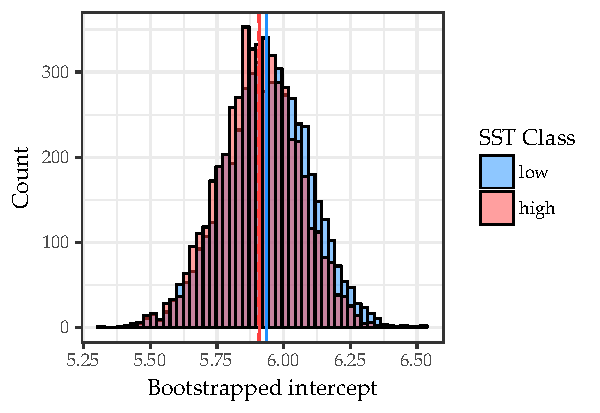
\includegraphics[width=0.45\textwidth]{./images/natl_boot_inter}
		\label{fig:natl-boot-inter}%
		}%
	\subfloat[Q-Q plot to compare the intercepts]{%
		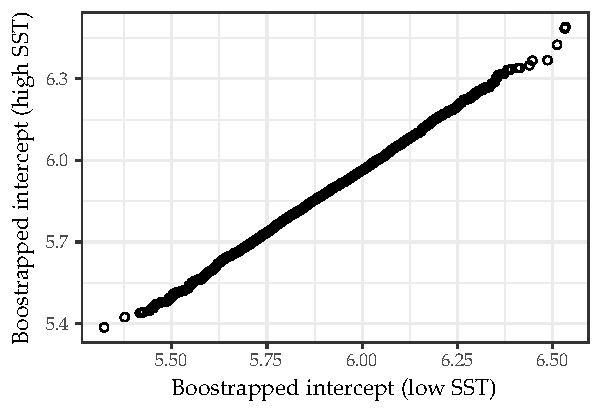
\includegraphics[width=0.45\textwidth]{./images/natl_boot_inter_qq}
		\label{fig:natl-boot-inter-qq}%
		}%
	\\
	\subfloat[Histogram of the bootstrapped slope]{%
		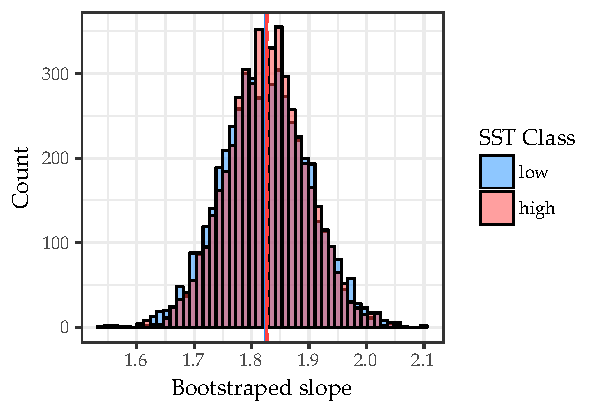
\includegraphics[width=0.45\textwidth]{./images/natl_boot_slope}
		\label{fig:natl-boot-slope}%
		}%
	\subfloat[Q-Q plot to compare the slopes]{%
		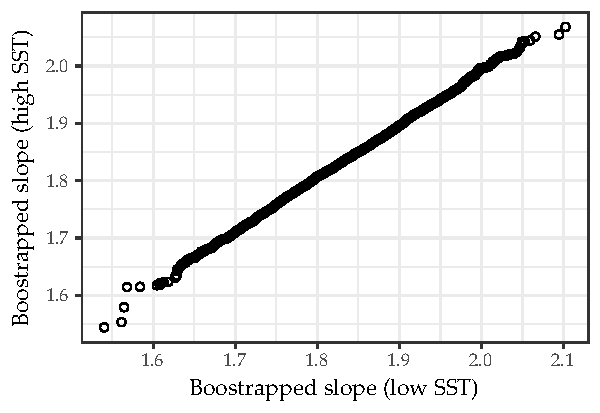
\includegraphics[width=0.45\textwidth]{./images/natl_boot_slope_qq}
		\label{fig:natl-boot-slope-qq}%
		}%
	\caption[Resampled slopes and intercepts obtained by bootstrapping for the North Atlantic basin data for the $PDI(\text{lifetime})$ regression model]{Resampled slopes and intercepts obtained by bootstrapping for the North Atlantic basin data for the $PDI(\text{lifetime})$ regression model. The dashed lines represent the coefficient estimates obtained via bootstrap, while the solid lines the estimates obtained via OLS}
	\label{fig:natl-boot-coefs}
\end{figure}

The coefficient estimates obtained for each of the four resulting regression models for the North Atlantic data are shown in \Cref{tab:natl-boot-coefs}. When compared to \Cref{tab:natl-ols-coefs} (coefficients obtained using OLS), one sees that the nominal values, as well as their standard error are almost identical.

This is by no means a bad thing. The main point of using bootstrap to resample the observations of hurricane occurrences was to have a robust theory to ensure the assumptions required for the linear model hold.

\begin{table}[H]
	\centering
	\begin{tabular}{cccccc}
		\toprule
		\toprule
		$X$ & $Y$ & SST class & $\hat{\beta}_{0}^{\ast}$ & $\hat{\beta}_{1}^{\ast}$ & $R^{2\ast}$ \\
		\midrule
		\multirow{2}{*}{lifetime} & \multirow{2}{*}{$PDI$}
		 & Low  & \num{ 5.91 \pm 0.17} & \num{1.84 \pm 0.08} & \num{0.67 \pm 0.03} \\
		&& High & \num{ 5.90 \pm 0.15} & \num{1.83 \pm 0.07} & \num{0.61 \pm 0.03} \\
		\midrule
		\multirow{2}{*}{$PDI$} & \multirow{2}{*}{lifetime}
		 & Low  & \num{-1.44 \pm 0.15} & \num{0.36 \pm 0.02} & \num{0.67 \pm 0.03} \\
		&& High & \num{-1.15 \pm 0.14} & \num{0.34 \pm 0.01} & \num{0.62 \pm 0.03} \\
		\bottomrule
	\end{tabular}
	\caption{Linear regression coefficients obtained performing bootstrap on the North Atlantic basin data}
	\label{tab:natl-boot-coefs}
\end{table}

The values of the test statistics calculated using the coefficient estimates obtained using bootstrap for this basin are shown in \Cref{tab:base-natl-boot-statistics}. The results, save some small discrepancies in the $\text{lifetime}(PDI)$ regression model, are comparable to those displayed in \Cref{tab:base-natl-ols-statistics}.
\begin{table}[H]
	\centering
	\begin{tabular}{cccccccc}
	\toprule
	\toprule
	$X$   & $Y$   & $T^{(1)}$ & $T^{(2)}$ & $T^{(3)}$ & $T^{(4)}$ & $T^{(5)}$ & $T^{(6)}$ \\
	\midrule
	lifetime & $PDI$ & $0.007$ & $0.007$ & $0.054$ & $0.031$ & $0.065$ & $0.095$ \\
	$PDI$ & lifetime & $0.289$ & $0.027$ & $0.048$ & $1.404$ & $1.324$ & $2.727$ \\
	\bottomrule
	\end{tabular}
	\caption{~Value of the studied statistics for North Atlantic basin data set using bootstrap}
	\label{tab:base-natl-boot-statistics}
\end{table}

%-----------------------------------------------------------------
\bigskip
For the Northeast Pacific basin data, we also observe normality in the bootstrapped coefficients, as can be seen in \Cref{fig:epac-boot-coefs}. A major difference, that we did not see in \Cref{fig:natl-boot-coefs} is that the distributions associated to low-SST and high-SST years present very distinct shapes, but this is a result of the inherent properties of the data; it represents the same numerical difference we already saw in the OLS coefficient estimates shown in \Cref{tab:epac-ols-coefs}), but from a graphical point of view.

\begin{figure}[H]
	\centering
	\subfloat[Histogram of the bootstrapped intercept]{%
		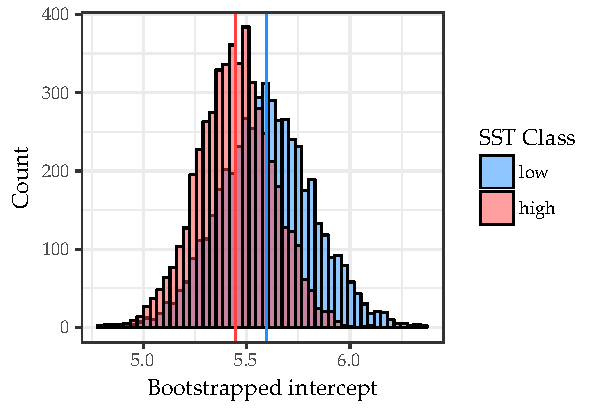
\includegraphics[width=0.45\textwidth]{./images/epac_boot_inter}
		\label{fig:epac-boot-inter}%
		}%
	\subfloat[Q-Q plot to compare the intercepts]{%
		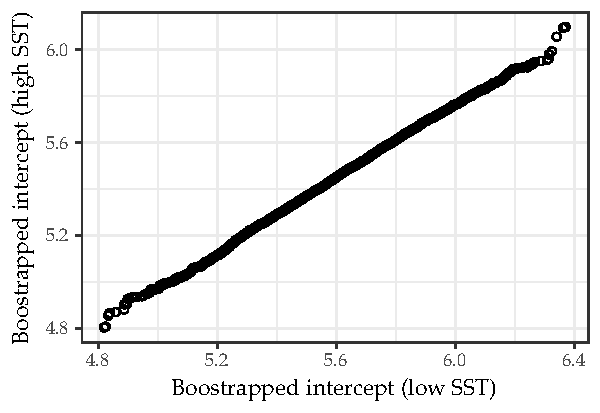
\includegraphics[width=0.45\textwidth]{./images/epac_boot_inter_qq}
		\label{fig:epac-boot-inter-qq}%
		}%
	\\
	\subfloat[Histogram of the bootstrapped slope]{%
		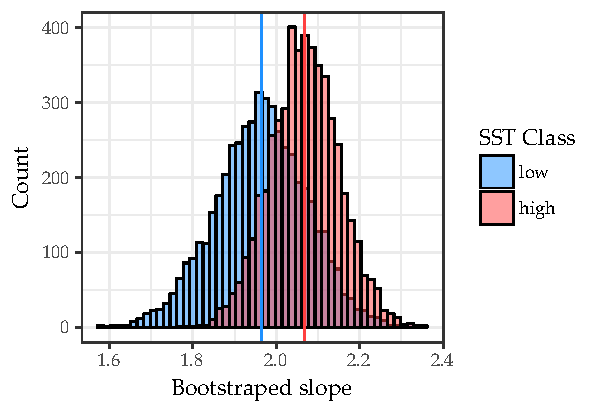
\includegraphics[width=0.45\textwidth]{./images/epac_boot_slope}
		\label{fig:epac-boot-slope}%
		}%
	\subfloat[Q-Q plot to compare the slopes]{%
		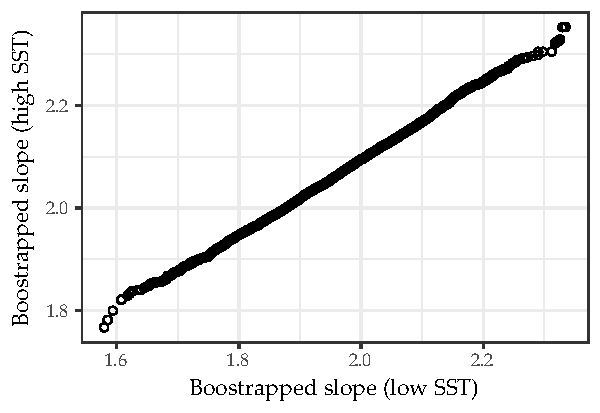
\includegraphics[width=0.45\textwidth]{./images/epac_boot_slope_qq}
		\label{fig:epac-boot-slope-qq}%
		}%
	\caption[Resampled slopes and intercepts obtained by bootstrapping for the Northeast Pacific basin data for the $PDI(\text{lifetime})$ regression model]{Resampled slopes and intercepts obtained by bootstrapping for the Northeast Pacific basin data for the $PDI(\text{lifetime})$ regression model. The dashed lines represent the coefficient estimates obtained via bootstrap, while the solid lines the estimates obtained via OLS}
	\label{fig:epac-boot-coefs}
\end{figure}

% \todo[inline]{Talk about coefficients of the linear regression}
The coefficient estimates obtained for each of the four resulting regression models for the Northeast Pacific data are shown in \Cref{tab:epac-boot-coefs}. When compared to \Cref{tab:epac-ols-coefs} (coefficients obtained using OLS), one sees that the nominal values, as well as their standard error are almost identical, just as happened for the North Atlantic data.

\begin{table}[H]
	\centering
	\begin{tabular}{cccccc}
		\toprule
		\toprule
		$X$ & $Y$ & SST class & $\hat{\beta}_{0}^{\ast}$ & $\hat{\beta}_{1}^{\ast}$ & $R^{2\ast}$ \\
		\midrule
		% \cmidrule(l){2-5}
		\multirow{2}{*}{lifetime} & \multirow{2}{*}{$PDI$}
		 & Low  & \num{ 5.59 \pm 0.24} & \num{1.97 \pm 0.12} & \num{0.60 \pm 0.05} \\
		&& High & \num{ 5.44 \pm 0.18} & \num{2.07 \pm 0.08} & \num{0.57 \pm 0.04} \\
		\midrule
		\multirow{2}{*}{$PDI$} & \multirow{2}{*}{lifetime}
		 & Low  & \num{-0.84 \pm 0.17} & \num{0.30 \pm 0.02} & \num{0.60 \pm 0.05} \\
		&& High & \num{-0.56 \pm 0.14} & \num{0.28 \pm 0.01} & \num{0.57 \pm 0.04} \\
		\bottomrule
	\end{tabular}
	\caption{Linear regression coefficients obtained performing bootstrap on the Northeast Pacific basin data}
	\label{tab:epac-boot-coefs}
\end{table}

The values of the test statistics calculated using the coefficient estimates obtained using bootstrap for this basin are shown in \Cref{tab:base-epac-boot-statistics}. The results are comparable and almost identical to those displayed in \Cref{tab:base-epac-ols-statistics}.

\begin{table}[H]
	\centering
	\begin{tabular}{cccccccc}
	\toprule
	\toprule
	$X$   & $Y$   & $T^{(1)}$ & $T^{(2)}$ & $T^{(3)}$ & $T^{(4)}$ & $T^{(5)}$ & $T^{(6)}$ \\
	\midrule
	lifetime & $PDI$ & $0.152$ & $0.103$ & $0.030$ & $0.509$ & $0.728$ & $1.237$ \\
	$PDI$ & lifetime & $0.286$ & $0.028$ & $0.027$ & $1.266$ & $1.266$ & $2.532$ \\
	\bottomrule
	\end{tabular}
	\caption{~Value of the studied statistics for Northeast Pacific basin data set using bootstrap}
	\label{tab:base-epac-boot-statistics}
\end{table}

\bigskip
% I summary, one can notice that the value of some of the $T^{(i)}$ statistics seem a bit high, both when performing a standard (OLS) regression analysis or a bootstrap-powered regression analysis. The problem is there is no way to quantify how big these statistics can be from theory.

% It is for this reason that we should perform a permutation test on the data following the methodology explained in \Cref{ssec:perm-test-theory}. This would allow us to properly test the hypothesis that
% \begin{align}
% 	f(Y \mid X = x)_{\text{low}} = f(Y \mid X = x)_{\text{high}}
% 	\tag{\ref{eq:hypothesis} ter}
% 	.
% \end{align}
